\documentclass{ds-report}
\assignment{Google App Engine} % Set to `Java RMI`, `Java EE` or `Google App Engine`.
\authorOne{Dries Janse} % Name of first team partner.
\studentnumberOne{r0627054} % Student number of first team partner.
\authorTwo{Steven Ghekiere} % Name of second team partner.
\studentnumberTwo{r0626062}  % Student number of second team partner.
\usepackage{graphicx}

\begin{document}
	\maketitle

	\paragraph{1. Which hosts/systems execute which processes, i.e. how are the remote objects distributed over hosts, if run in a real deployment on the App Engine platform (not a lab deployment where everything runs on the same machine)? Clearly outline which parts belong to the front- and backend. Create a component/deployment diagram to illustrate this: highlight where the client and server are.} \mbox{}\\\\
Figure \ref{fig:deployment_diagram} shows the deployment diagram of the application. This diagram shows how the different classes can be deployed in a real distributed deployment.



	
	\paragraph{2. At which step of the workflow for booking a car reservation (create quote, collect quotes, confirm quotes) would the indirect communication between objects or components kick in? Describe the steps that cause the indirect communication, and what happens afterwards.} \mbox{}\\\\
The indirect communication takes place at the 'confirm quotes' step in our application. The actual confirmation and creation of the reservations is the most demanding process. This part is the bottleneck activity of the application. By decoupling this part of the application, it allows the  back-end to introduce an additional delay for the processing. The front-end will achieve better availability and performance because it does not have to wait for the actual creation of the reservations. The CarRentalModel, which contains the confirmQuotes method, will push a task to the task queue service. The task queue service will then send a http post request to the worker with the worker url and the serialized parameters. The worker will execute the task. In this case it tries to create reservations for all the quotes, making use of a transaction.


	\paragraph{3. Which kind of data is passed between the front- and back-end? Does it make sense to persist data and only pass references to that data?} \mbox{}\\\\
Instances of the 'PayloadWrapper' class are passed between the front- and back-end. This class has a list of quotes, the name of the renter and the email of the renter. The confirmQuotes method in the CarRentalModel class will create an instance of the PayloadWrapper class. This instance will be serialized to a byte array and given to a TaskOptions object. This TaskOptions object will be pushed to a queue and the worker will execute the task.




	\paragraph{4. How have you implemented your backchannel? What triggers the backchannel to be used, how does the client use the backchannel and what information is sent?} \mbox{}\\\\





	\paragraph{5. How does your solution to indirect communication improve scalability?} \mbox{}\\\\


		\paragraph{6. Workers in GAE’s Task Queues are by default set to run in parallel. While parallelism is usually a desirable property of a cloud service, as it enables scalability and thus faster overall processing, it may also endanger the application’s state consistency. Assume a scenario in which two different clients try to confirm a couple of tentative reservations, i.e. their quotes are queued to be processed by the back end. Both include a tentative reservation for the last available car of a certain car type, so that, assuming correct behaviour of the car rental application, it should fail to confirm the quotes for one of them.} \mbox{}\\\\


 

	\paragraph{7.  How does using a NoSQL database affect scalability and availability?} \mbox{}\\\\




	\paragraph{8. How have you structured your data model (i.e. the entities and their relationships)? Compared to a relational database, what sort of query limitations have you faced when using the Cloud Datastore?} \mbox{}\\\\


	\paragraph{9. What is the most critical difference between confirmQuote and confirmQuotes from the viewpoint of transaction management? Explain an alternative to your solution for the all-or-nothing semantics of confirmQuotes which is essentially different from the viewpoint of transaction management. Given the underlying distributed storage layer, what are the implications of each solution for performance and data consistency?} \mbox{}\\\\
	
		\clearpage

\begin{figure}
  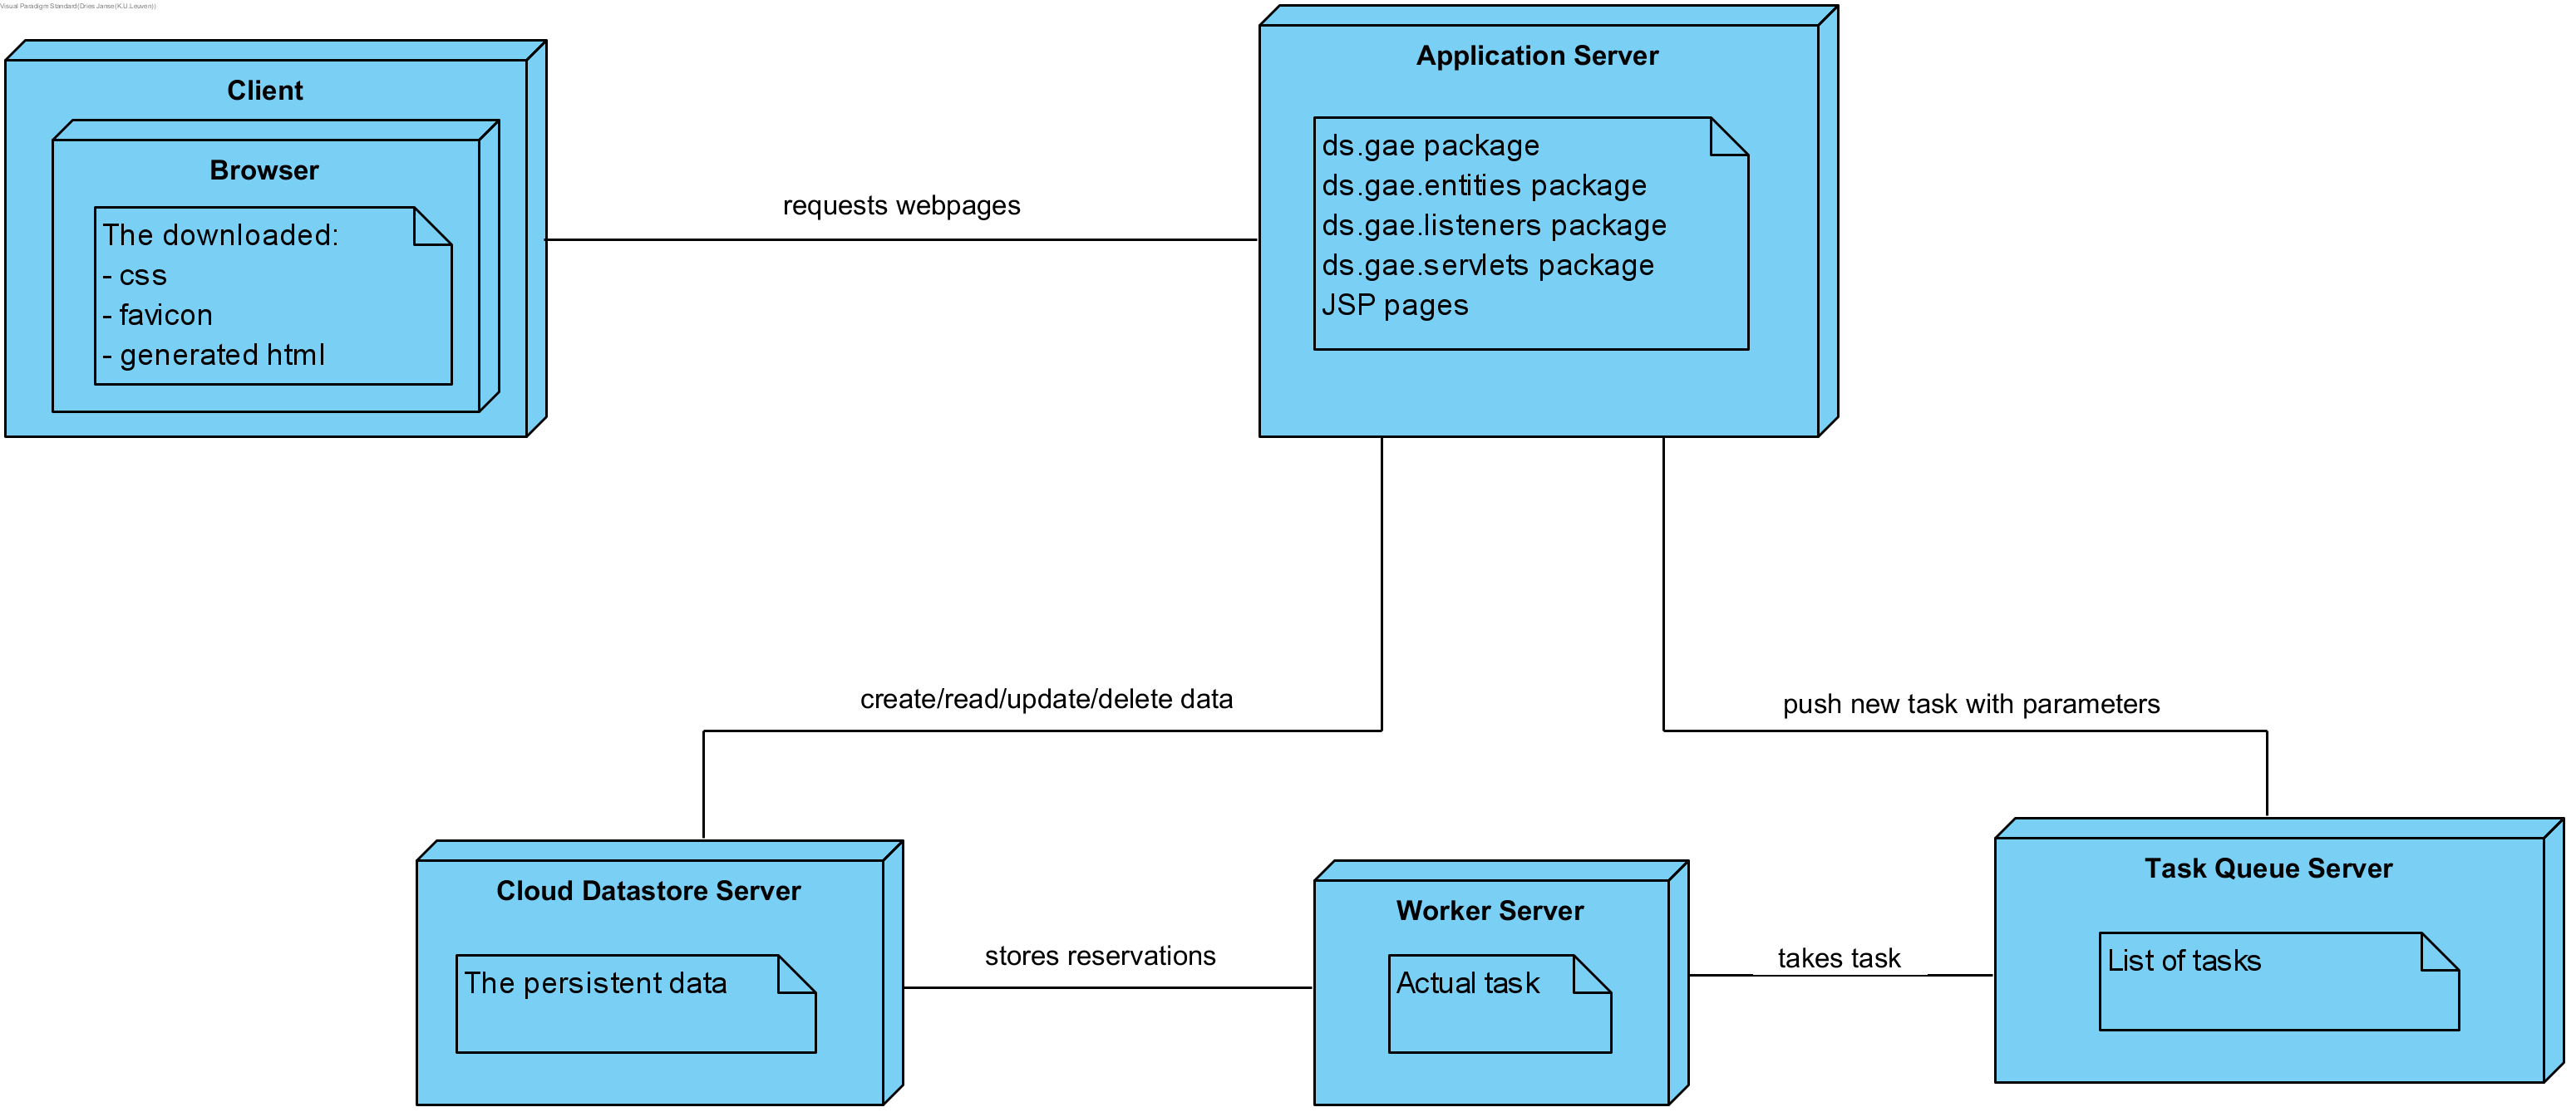
\includegraphics[width=\linewidth]{GAE_opdracht_2_deployment.png}
  \caption{Deployment diagram}
  \label{fig:deployment_diagram}
\end{figure}	

	
	\clearpage


	% You can include diagrams here.
	
\end{document}